\documentclass[crop,tikz,pgf]{standalone}% 'crop' is the default for v1.0, before it was 'preview'
\usetikzlibrary{calc}
\begin{document}
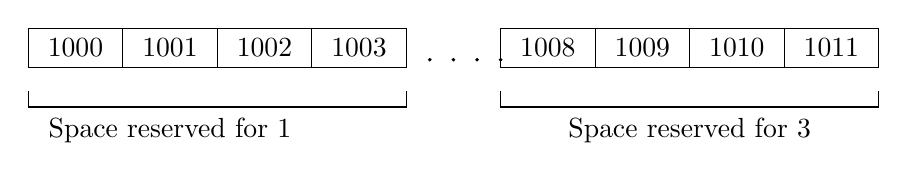
\begin{tikzpicture}
  \foreach \x in {0, ..., 3}
  \draw (\x*1.2cm, 0) -- +(1.2cm, 0) -- +(1.2cm, 0.5cm) -- +(0, .5cm) --
  cycle;
  \node at(5.1cm, .1cm) [circle,fill,inner sep=.5pt](a){};
  \node at(5.4cm, .1cm) [circle,fill,inner sep=.5pt](a){};
  \node at(5.7cm, .1cm) [circle,fill,inner sep=.5pt](a){};
  \node at(6cm, .1cm) [circle,fill,inner sep=.5pt](a){};
  \foreach \x in {0, ..., 3}
  \draw (\x*1.2cm+6cm, 0) -- +(1.2cm, 0) -- +(1.2cm, 0.5cm) -- +(0, .5cm) --
  cycle;
  \foreach \x [evaluate=\x as \xeval using \x+1000] in {0, ..., 3} 
  \node at(\x*1.2cm + .6cm, .25cm) {\pgfmathtruncatemacro{\yet}{\xeval}\yet};
  \foreach \x [evaluate=\x as \xeval using \x+1008] in {0, ..., 3} 
  \node at(\x*1.2cm+6.6cm, .25cm) {\pgfmathtruncatemacro{\yet}{\xeval}\yet};

  \draw (0, -.3cm) -- (0, -.5cm) -- (4.8cm, -.5cm) -- (4.8cm, -.3cm);
  \draw (6cm, -.3cm) -- (6cm, -.5cm) -- (10.8cm, -.5cm) -- (10.8cm, -.3cm);

  \node at (1.8cm, -.8cm) {Space reserved for 1};
  \node at (8.4cm, -.8cm) {Space reserved for 3};
  
  %  \draw (0.2cm, 0.6cm) -- (0.2cm, 1cm);
%  \draw (0.6cm, 0.6cm) -- (0.6cm, 1cm) -- (3.4cm, 1cm) -- (3.4cm, 0.6cm);
%  \draw (3.8cm, 0.6cm) -- (3.8cm, 1cm) -- (12.6cm, 1cm) -- (12.6cm, 0.6cm);
%  \foreach \x in {31, ..., 0}
%  \node at (\x*0.4cm, 0) [xshift=.2cm, yshift=-.3cm, align=center] {\tiny \x};
%  \node at (0.2cm, 1.3cm) [align=center] {sign};
%  \node at (2cm, 1.3cm) [align=center] {exponent(8 bits)};
%  \node at (8.2cm, 1.3cm) [align=center] {fraction(23 bits)};
\end{tikzpicture}
\end{document}
